
\kwc{This chapter provides the background knowledge necessary for understanding the subsequent chapters. 
Readers may choose one or more sections to read for a particular chapter or skip the sections they are familiar with.
Section~\ref{sec:bg_gnn} introduces GNNs, which are the focus of \cref{ch:hector,ch:pytorch_direct}.
Section~\ref{sec:bg_transformers} delves into transformers, offering context for Chapter~\ref{ch:ssdtrain}.
Section~\ref{sec:bg_cuda} covers the architecture, programming model, programming interface and compilation flow for Nvidia GPUs.
Section~\ref{sec:bg_python} overviews the Python language.
Section~\ref{sec:bg_pytorch} introduces the PyTorch computing stack.

}

\section{Graph Neural Networks}
\label{sec:bg_gnn}
Inspired by the success of convolutional neural networks~(CNNs)~\cite{CNN0}, people devised GNNs as a new type of neural network that applies similar filters to graphs~\cite{lecunGCN, hamilton2017inductive, Pinterest, GCNPierre, kipf2016semi, kipf2016variational, pmlr-v48-niepert16}.
While CNNs excel at extracting features from grid-like data such as images, GNNs are designed to propagate and transform features according to the structure of graphs, allowing them to retain relational information between entities represented by nodes and edges.
GNNs are increasingly applied in diverse domains, including social network analysis and recommender systems~\cite{hamilton2017inductive,Pinterest,kipf2016semi}, etc.


GNNs have shown significant advantages in graph representation learning~\cite{HamiltonYL17, hamilton2017inductive, Pinterest}, where the goal is to embed graph-structured information into low-dimensional dense vectors.
The trained model can produce vectors for specified nodes or edges. Then, tasks\kwc{, e.g., node classification, link prediction, etc.,} can be performed by only relying on them rather than all the raw data in the graph, e.g., the adjacency list, node features, etc. 
As Hamilton et al.\ \cite{HamiltonYL17} noted, traditional algorithms, e.g., DeepWalk~\cite{DeepWalk} and node2vec~\cite{node2vec}, cannot generalize to perform inference on unseen nodes or edges during training, and their representation power is limited.
In comparison, GNNs offer a more powerful and flexible approach, capable of addressing these limitations and enabling inductive learning for new graph data.
\kwa{(Paragraph moved.)}


A widely-used GNN model is graph convolutional network~(GCN)~\cite{kipf2016semi}.
Formally, a GCN layer is defined as 
$    \overrightarrow{{h}^{(l+1)}} = \sigma\left(A^{*}\overrightarrow{{h}^{(l)}}W^{(l)}\right)$
, where $W^{(l)}$ denotes the trainable weight matrix of the $l$-th layer, $\sigma$ is a non-linear activation function and $\overrightarrow{{h}^{(l)}}$ is the node representation at layer $l$. In particular, the node input features are denoted as $\overrightarrow{h^{(0)}}$. $A^{*}$ is the adjacency matrix normalized by node degrees:

\begin{equation*}
A^{*}_{i,j}=
\begin{cases}
\frac{1}{\sqrt{d_{out,j}}\cdot\sqrt{d_{in,i}}}, &\text{if there is an edge from } j \text{ to } i\\
0, &\text{otherwise}
\end{cases}
\end{equation*}

where $d_{out,j}$ is node $j$'s out degree and $d_{in,i}$ is the in degree of node $i$.




\begin{figure}[!tb]
\centering
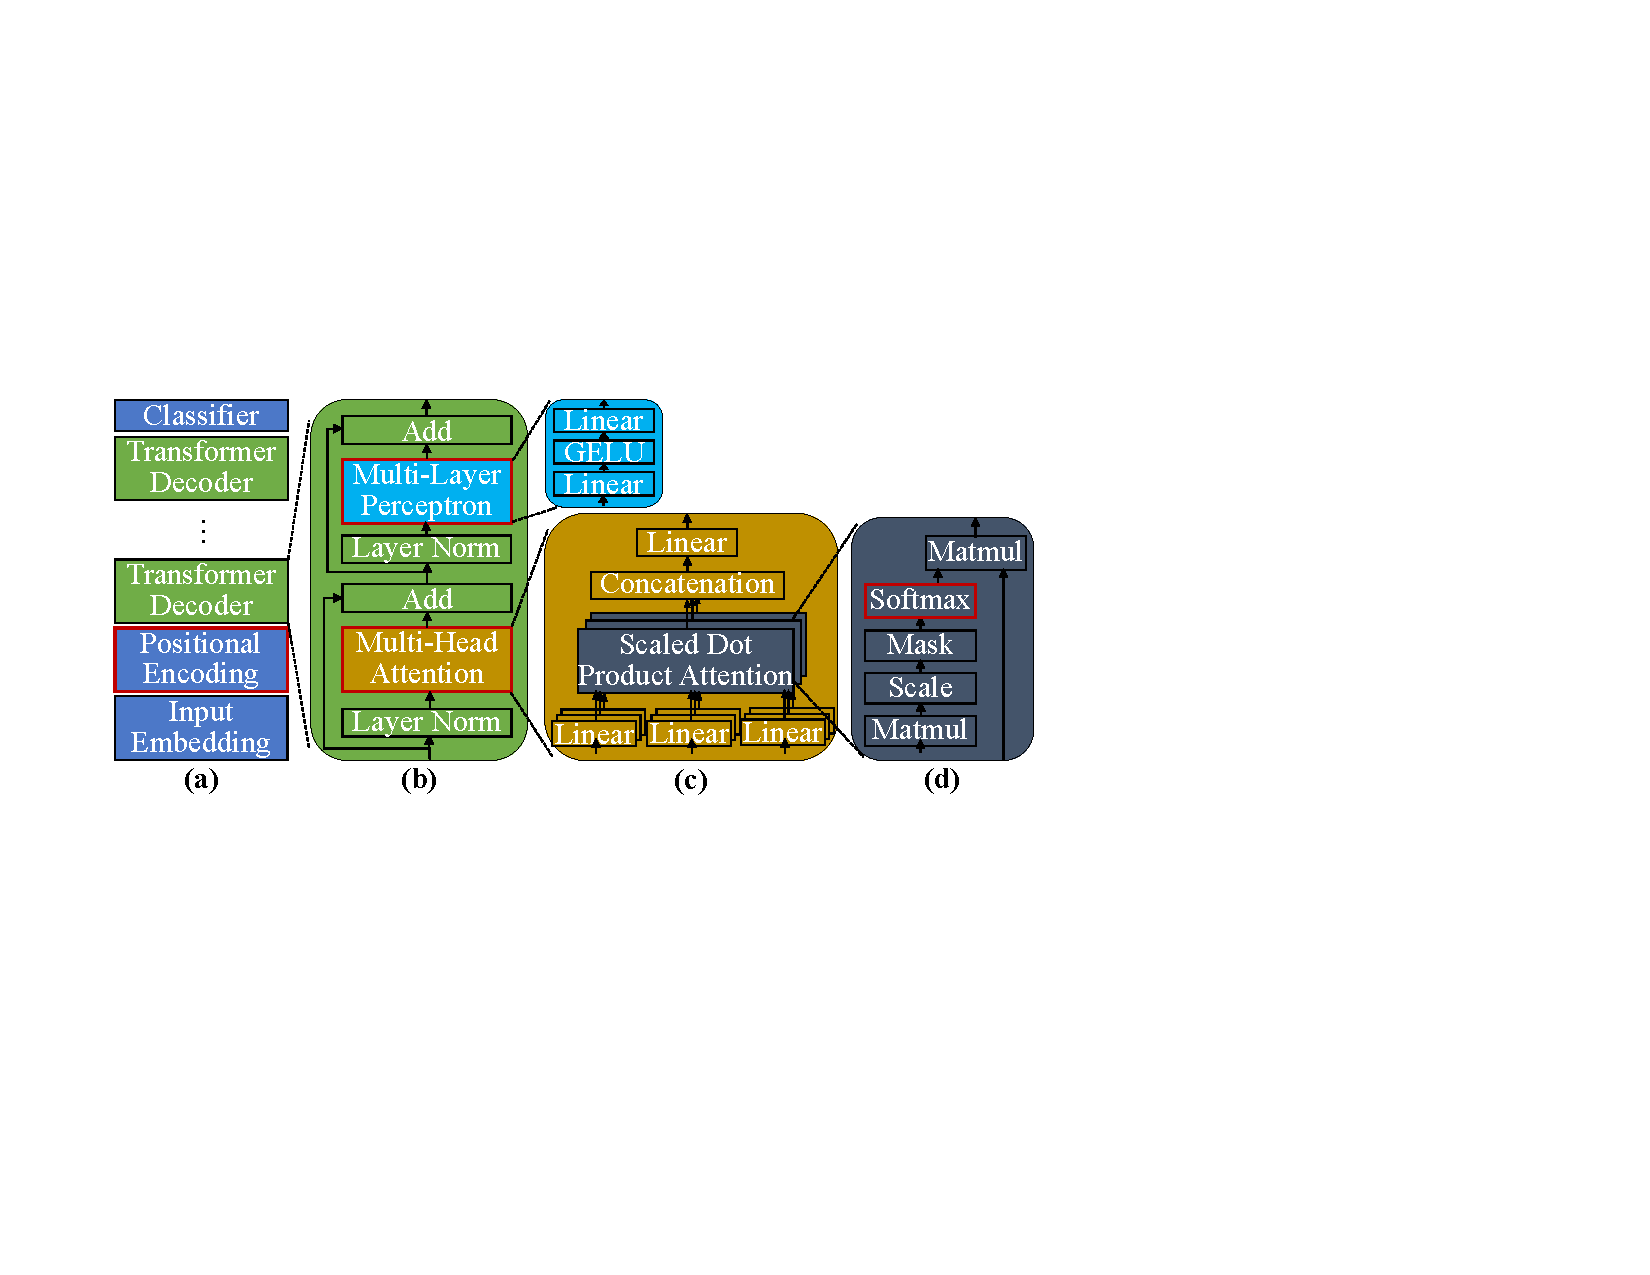
\includegraphics[width=0.8\linewidth]{figures/SSDTrain/transformer_compact.pdf}
\caption{\label{fig:transformer} Hierarchical breakdown of the GPT model. In training, dropout is applied to the output of each layer with red borders.}
\end{figure}



\section{Transformer-Based Large Language Models}
\label{sec:bg_transformers}

LLMs now drive a wide range of applications, including chatbots~\cite{openaiChatGPT2022}, search~\cite{BingChatMicrosoft2023}, content generation~\cite{midjourneyMidjourney2022}, reasoning~\cite{langchainLangChain2022}, etc. These models, when sufficiently large in size, demonstrate emergent abilities~\cite{weiEmergentAbilitiesLarge2022} and thus the ability to handle complicated tasks. \kwc{Consequently, LLMs today can be as large as containing hundreds of billions of parameters. Furthermore,} model designers \kwc{are driven to} continue to scale up the size of LLMs, carrying more parameters. %


Most LLM architectures, including GPT~\cite{radfordLanguageModelsAre2019},  are transformer-based~\cite{vaswaniAttentionAllYou2017}. As Figure~\ref{fig:transformer}(a) shows, the GPT model consists mainly of multiple transformer layers. Before transformer layers, GPT takes in the tokenized text and maps the tokens into dense vectors with positional information. The task determines the last part of the model architecture.
For instance, a classifier could be added for text classification tasks.
Figure~\ref{fig:transformer}(b) shows that each transformer layer is primarily made up of an attention block and a multi-layer perception~(MLP) block. Attention blocks~(Figure~\ref{fig:transformer}(c)) compute a weight, called attention, for each token pair, and produce dense vectors for each token via weighted summation. The MLP blocks transform the vector of each token into a new vector.




GPT is a decoder-only model because it only involves transformer decoder layers. A transformer encoder layer has the same structure as the transformer decoder layer except that the latter imposes causality on the attention mask in Figure~\ref{fig:transformer}(d): the causal mask ensures that the new vectors produced by the attention block for each token depend only on vectors of tokens, not after this token. By this categorization, transformer models are classified as (1)~encoder-only, e.g., BERT~\cite{devlinBERTPretrainingDeep2019}, (2)~decoder-only, e.g., GPT, Llama~\cite{touvronLlamaOpenFoundation2023}, and (3)~encoder-decoder, e.g., T5~\cite{raffelExploringLimitsTransfer2023}. In encoder-decoder models, the transformer decoder layers take in both outputs from the encoders and another text and apply two attention blocks---the self-attention block is applied to the new text, and the cross-attention block is applied among the tokens in the sequence from the encoder and tokens in the new text. 


Parallelizing LLM training involves partitioning and/or replicating the model and the data into different GPUs~\cite{xuGSPMDGeneralScalable2021}. Pipeline parallelism, data parallelism, and model parallelism are the three levels of parallelism available to all LLM models and widely adopted in frameworks, e.g., Megatron, DeepSpeed, and PyTorch 2.0~\cite{shoeybiMegatronLMTrainingMultiBillion2020a,rasleyDeepSpeedSystemOptimizations2020,anselPyTorchFasterMachine2024}.
Pipeline parallelism partitions the model into several chunks of layers and places them on different GPUs. In a step, when the GPUs finish their layers, the output is passed to the GPUs owning the next layers.
Data parallelism replicates the models in different groups of GPUs and assigns separate micro-batches to each group.
At the end of a step, the gradients in each group are aggregated to update all the model replicas.
Model parallelism shards a weight tensor and puts shards onto different GPUs. Each GPU performs a part of the computation using its shard for the corresponding operator.
Given the system scale and interconnect, all or a few among the three levels may be used.
Zero Redundancy Optimizer~(ZeRO)~\cite{rajbhandariZeROMemoryOptimizations2020a} further reduces memory use with data parallelism by sharding the optimizer states, and/or optionally the gradients and parameters and stores the shards across these GPUs.


\section{Nvidia GPU Architectures and Programs}
\label{sec:bg_cuda}

While the CPU is designed to minimize the latency of each operation, the GPU is a massively parallel processor optimized to maximize throughput~\cite{PMPP4}. To support this computational parallelism, each GPU device is equipped with memory that has very high bandwidth, reaching an order of magnitude of TB/s after high-bandwidth memory~(HBM) is adopted. Just as each CPU chip contains multiple cores, each Nvidia GPU contains hundreds of cores, called streaming multiprocessors~(SMs). The structure of an SM is illustrated in Figure~\ref{fig:sm_arch}. In an SM, the scheduler selects instructions ready for execution, which are then dispatched by the dispatcher unit to various function units. The function units include floating-point units, arithmetic logic units~(ALUs), tensor cores, transcendental and data type conversion units~(XUs), and load-store units~(LSUs). LSUs are responsible for transferring data between the register file and memory, while the other function units operate on values stored in registers. For fast on-chip \kwc{memory}, each SM also contains its own L1 cache and a scratchpad, called shared memory.

A common way to program Nvidia GPUs with a parallel computing workload is to create a CUDA C++ program. Functions executed on Nvidia GPUs are called kernels. During the execution of a kernel, a massive number of threads execute the same logic specified in the kernel's CUDA C++ function definition. CUDA C++ well matches Nvidia GPUs' single instruction, multiple threads~(SIMT) execution model: At each time during execution, all threads that are being executed in an SM execute the same instruction. Threads within a CUDA kernel are organized into blocks, and each block is scheduled onto one SM, where it remains until all threads within the block finish executing. To hide latency, programmers typically aim for high occupancy, i.e., ensuring that each SM is assigned a large number of threads.


The Nvidia compiler, nvcc, compiles CUDA kernels into the PTX~(Parallel Thread Execution) intermediate language. The machine code executed by the GPU is in a proprietary instruction set architecture~(ISA), called SASS~(Streaming ASSembler). Translation from PTX to SASS can occur at compile time or runtime via the GPU driver.


\begin{figure}[]
    \centering
    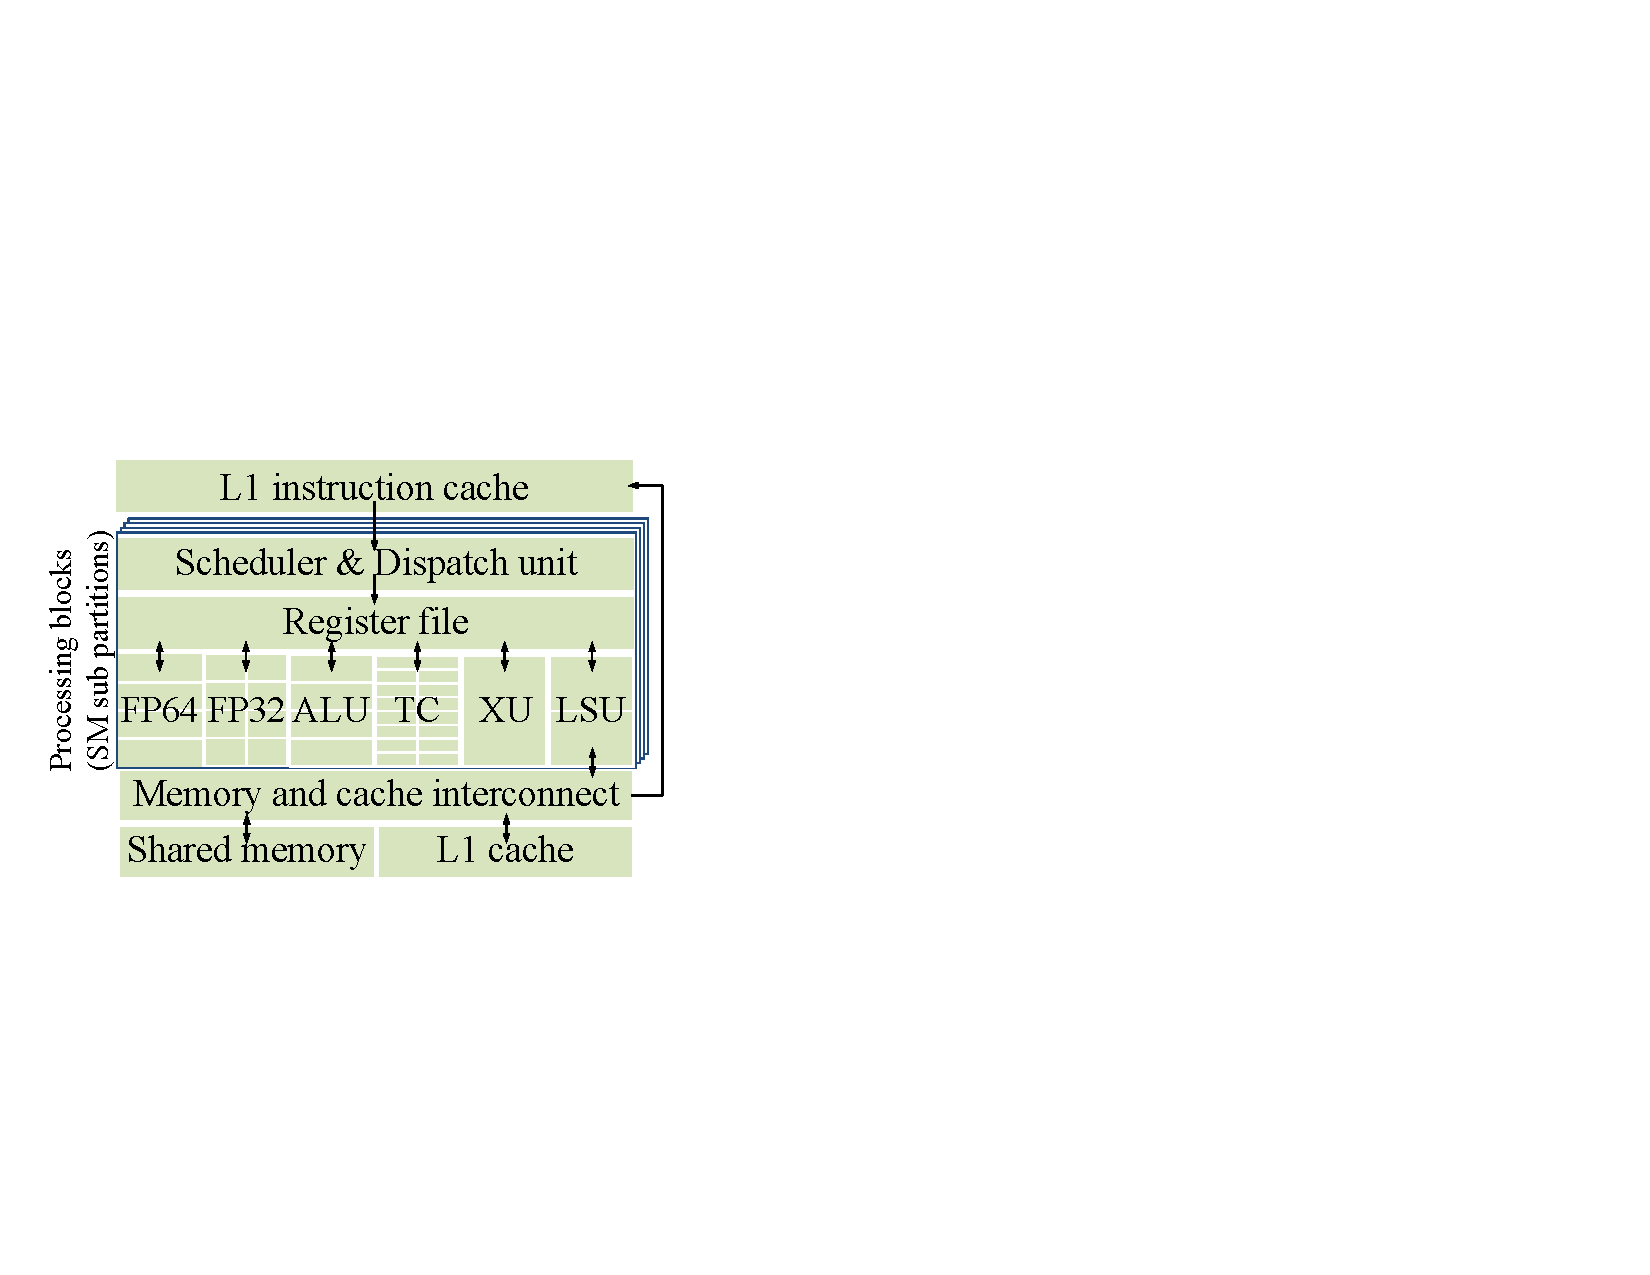
\includegraphics[width=0.45\linewidth]{figures/Intro/sm_arch.pdf}
    \caption{Structure of a streaming multiprocessor~(SM) in an Nvidia Volta V100 GPU~\cite{V100Whitepaper,jiaDissectingNVIDIAVolta2018,nickollsInstructionsManagingParallel2019,davidm.koppelmanEE7722GPU2023,nvidiaKernelProfilingGuide2024}. The execution units include FP64 units, FP32 units, arithmetic logic units~(ALUs), tensor cores~(TCs), transcendental and data type conversion units~(XUs), and load-store units~(LSUs). }
    \label{fig:sm_arch}
\end{figure}


\section{The Python Language}
\label{sec:bg_python}

People in the deep learning community use Python extensively. Python is easy to use due to its simplicity, expressiveness, and powerful features. One of the key features of Python is its interpreter, so users do not need to compile their code before execution. Additionally, Python's dynamic typing, known as duck typing, frees programmers from declaring the type of each variable and allows variables to change types during execution, simplifying development. Python also features rich ecosystems with widely-used package managers, e.g., Python's built-in Pip, Anaconda, etc.

To illustrate how friendly Python is, we write a Python program to sort tuples in Listing~\ref{lst:sort_second_python}. In contrast, Listing~\ref{lst:sort_second_cpp} shows the C++ program doing the same job. Both programs sort the \texttt{records} variable according to each tuple's second element. The \texttt{records} variable stores the name and address of each person as a two-string tuple. The tuples will be sorted according to the second string, i.e., the addresses. Both programs execute three steps: 1)~defining the \texttt{records} variable, 2)~sorting, and 3)~printing the sorted records.


As shown, the Python code is more expressive and quicker to develop due to several factors. First, it does not need compilation and an entry point \texttt{main()} function. Second, Python does not require the type declaration of each variable. Third, Python has a simpler lambda function syntax and supports containers in the built-in \texttt{print()} function.


\begin{lstlisting}[float,caption={Python code to sort tuples according to their second elements.},label={lst:sort_second_python}]
# Step (1) Define the records variable
records = [("Alice", "227 CSL"), 
     ("Bob", "1210 Siebel Center"),
     ("Charlie", "2120 ECE Building")]
# Step (2) Sort the records
records.sort(key=lambda x: x[1])
# Step (3) Print results
print(records)
\end{lstlisting}

\begin{lstlisting}[float,language=C++,caption={C++ code to sort tuples by their second elements~\cite{geeksforgeeksSortingVectorTuple2020}.},label={lst:sort_second_cpp}]
#include <bits/stdc++.h>
using namespace std;
int main() {
   // Step (1) Define the records variable
   vector<tuple<string, string> > records{ 
      {"Alice", "227 CSL"}, 
      {"Bob", "1210 Siebel Center"},
      {"Charlie", "2120 ECE Building"}};
   // Step (2) Sort the records
   sort(records.begin(), records.end(), 
      [](auto a, auto b) {return get<1>(a) < get<1>(b);});
   // Step (3) Print results
   for (auto r: records) {
      cout << get<0>(r) << " " << get<1>(r) << "\n";}}
\end{lstlisting}


One of the biggest concerns of Python is the significant serialization penalty caused by the global interpreter lock~(GIL) in multithreading programs. As the most widely-used Python implementation, CPython~\cite{wikipediaCPython2008} uses GIL to ensure thread safety. To mitigate this, frameworks work around GIL. One method is to put performance-critical logic in the C++ framework libraries and release the GIL once the control flow goes outside the Python code~\cite{CanPytorchBypass2019}. Another direction is to remove the GIL from the Python implementation. Although there are some alternate GIL-free Python implementations~\cite{wikipediaIronPython2006} to CPython, many frameworks rely on CPython-specific implementation details, making it challenging to migrate these frameworks to such alternatives. These limitations led to the \kwc{Python Enhancement Proposal (PEP) 703} to make GIL optional~\cite{samgrossPEP703Making2023} in CPython, which has been accepted recently.


\begin{lstlisting}[float,caption={PyTorch code to define model in Figure~\ref{fig:pytorch_graph} and perform a training step. We denote the input hidden dimension as \texttt{IN\_DIM} and the output hidden dimension as \texttt{OUT\_DIM}.},label={lst:pytorch_nested_module}]
import torch
from torch.nn.parameter import Parameter
# Step (1) Define the nested module
class MyLinear(torch.nn.Module):
    def __init__(self):
        super(MyLinear, self).__init__()
        self.x = Parameter(torch.randn(IN_DIM, OUT_DIM))
        self.b = Parameter(torch.randn(OUT_DIM))
    def forward(self, inp):
        return torch.matmul(inp, self.x) + self.b
class MyLinearWithActivation(torch.nn.Module):
    def __init__(self):
        super(MyLinearWithActivation, self).__init__()
        self.linear = MyLinear()
        self.activation = torch.nn.Tanh()
    def forward(self, inp):
        return self.activation(self.linear(inp))
# Step (2) Define the deep learning model
linear_with_activation = MyLinearWithActivation()
loss_fn = torch.nn.MSELoss()
# Step (3) Execute a training step
y = linear_with_activation(x)
loss = loss_fn(y, y_expected)
loss.backward()
\end{lstlisting}

\section{The PyTorch Computing Stack}
\label{sec:bg_pytorch}

\begin{figure}[]
    \centering
    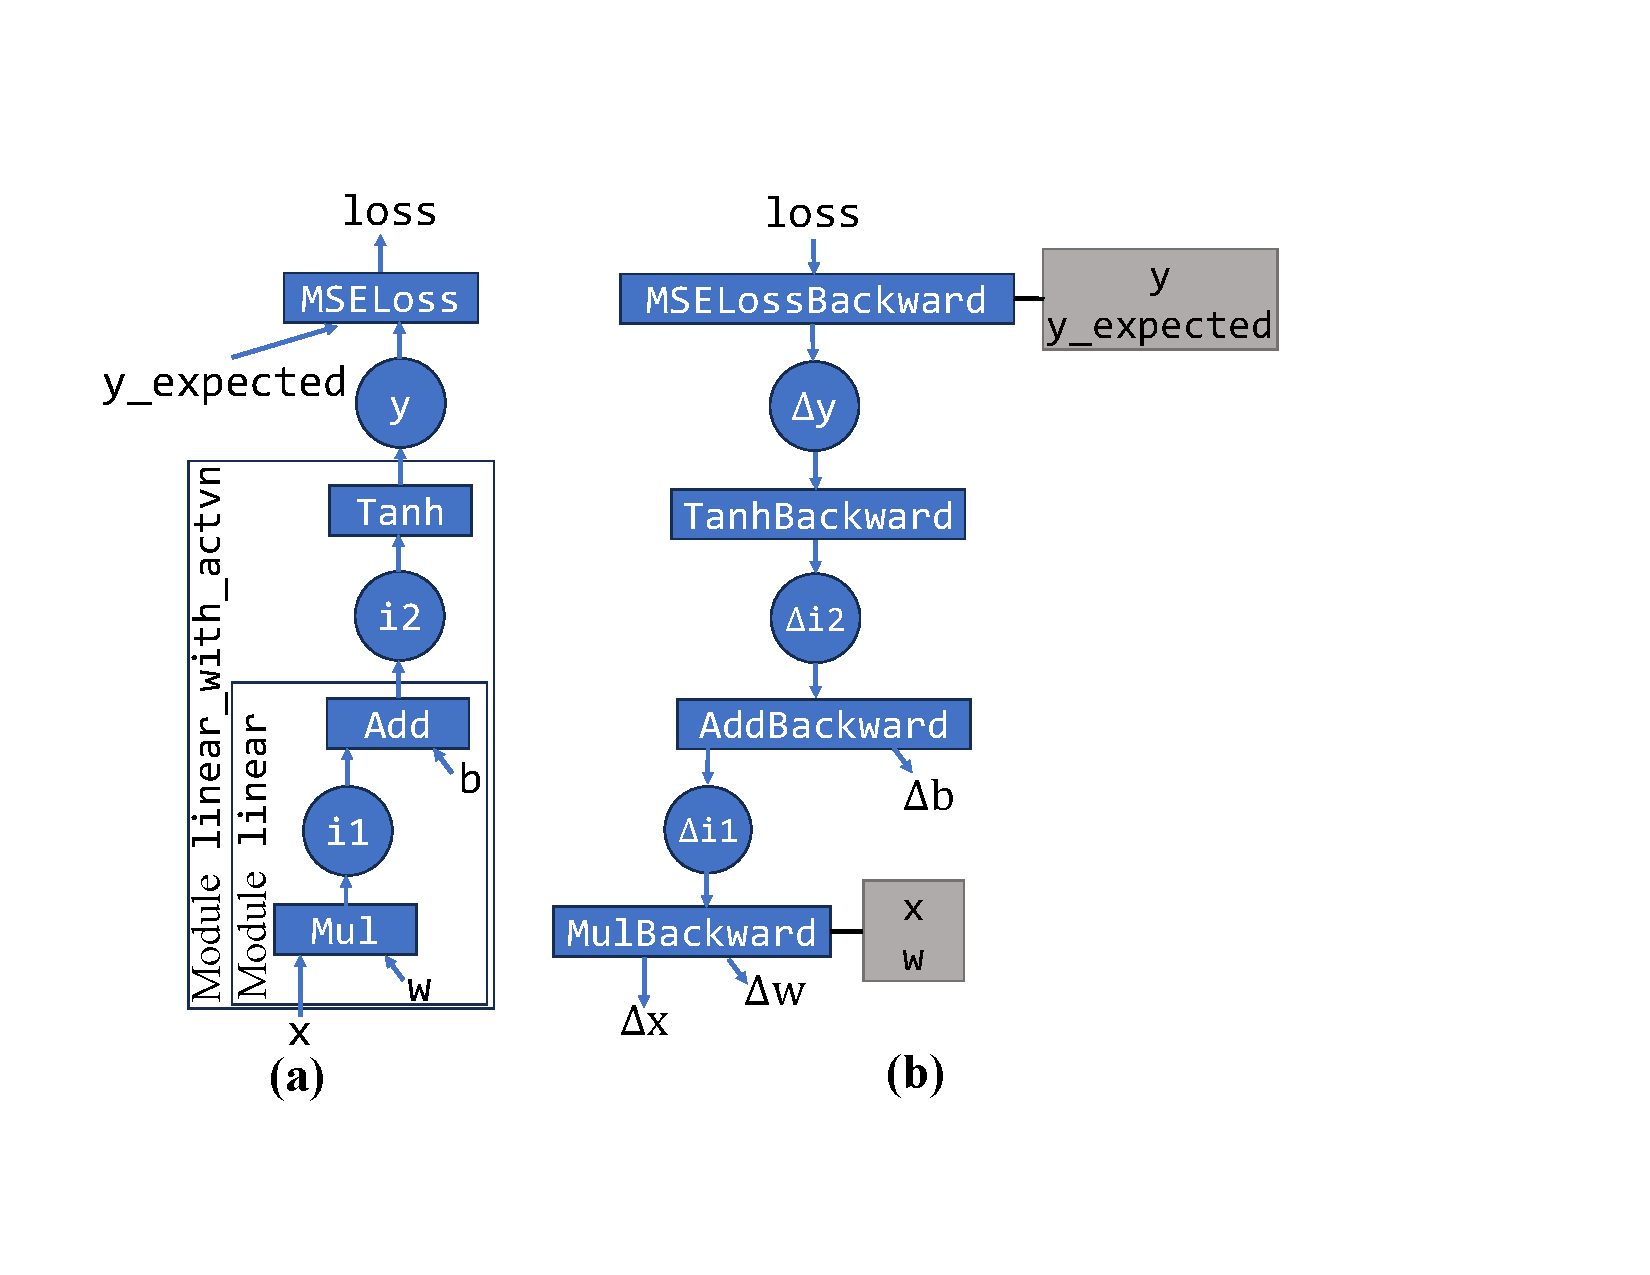
\includegraphics[width=0.65\linewidth]{figures/Intro/pytorch_graph_with_gradients.pdf}
    \caption{\kwc{Computational graphs of} (a)~forward propagation and (b)~backward propagation  for code in Listing~\ref{lst:pytorch_nested_module}. To compute gradients in backward propagation, dependent tensors are stored in the graph~(gray blocks with black text) during forward propagation. By default, PyTorch operates in eager mode and only constructs and stores the \kwc{graph of} backward propagation in memory during runtime. }
    \label{fig:pytorch_graph}
\end{figure}
Thanks to its intuitive, dynamic, and flexible programming interface, PyTorch is friendly to both users and developers who build packages on top of PyTorch. As a result, PyTorch has gained much popularity since its inception. 

By default, PyTorch executes code eagerly, meaning operations are computed immediately as they are called. For example, Listing~\ref{lst:pytorch_nested_module} defines a simple \kwc{classifier} model with mean squared error~(MSE) as the loss function and executes a training step.  The model contains a nested module, \texttt{linear\_with\_activation}, and a loss function \texttt{loss\_fn()}. \texttt{linear\_with\_activation} is made up of a linear layer and a hyperbolic tangent activation function. Figure~\ref{fig:pytorch_graph} illustrates both the forward-propagation and backward-propagation computational graphs for this example. As shown in step~(1) of Listing~\ref{lst:pytorch_nested_module}, the modules are defined as subclasses of \texttt{torch.nn.Module}. In the class definition, the initialization \kwc{method} \texttt{\_\_init\_\_()} initializes the parameters of layers and submodules. The \kwc{method} \texttt{forward()} defines the forward propagation logic of this module. Step~(2) constructs the model, consisting of the nested module \texttt{linear\_with\_activation} and the MSE loss function \texttt{loss\_fn}. Step~(3) executes a training step, i.e., one forward propagation and one backward propagation pass. \kwc{\texttt{x} is the input data, \texttt{y} is the predicted labels, and \texttt{y\_expected} is the ground-truth labels.}


\begin{figure}[!t]
    \centering
    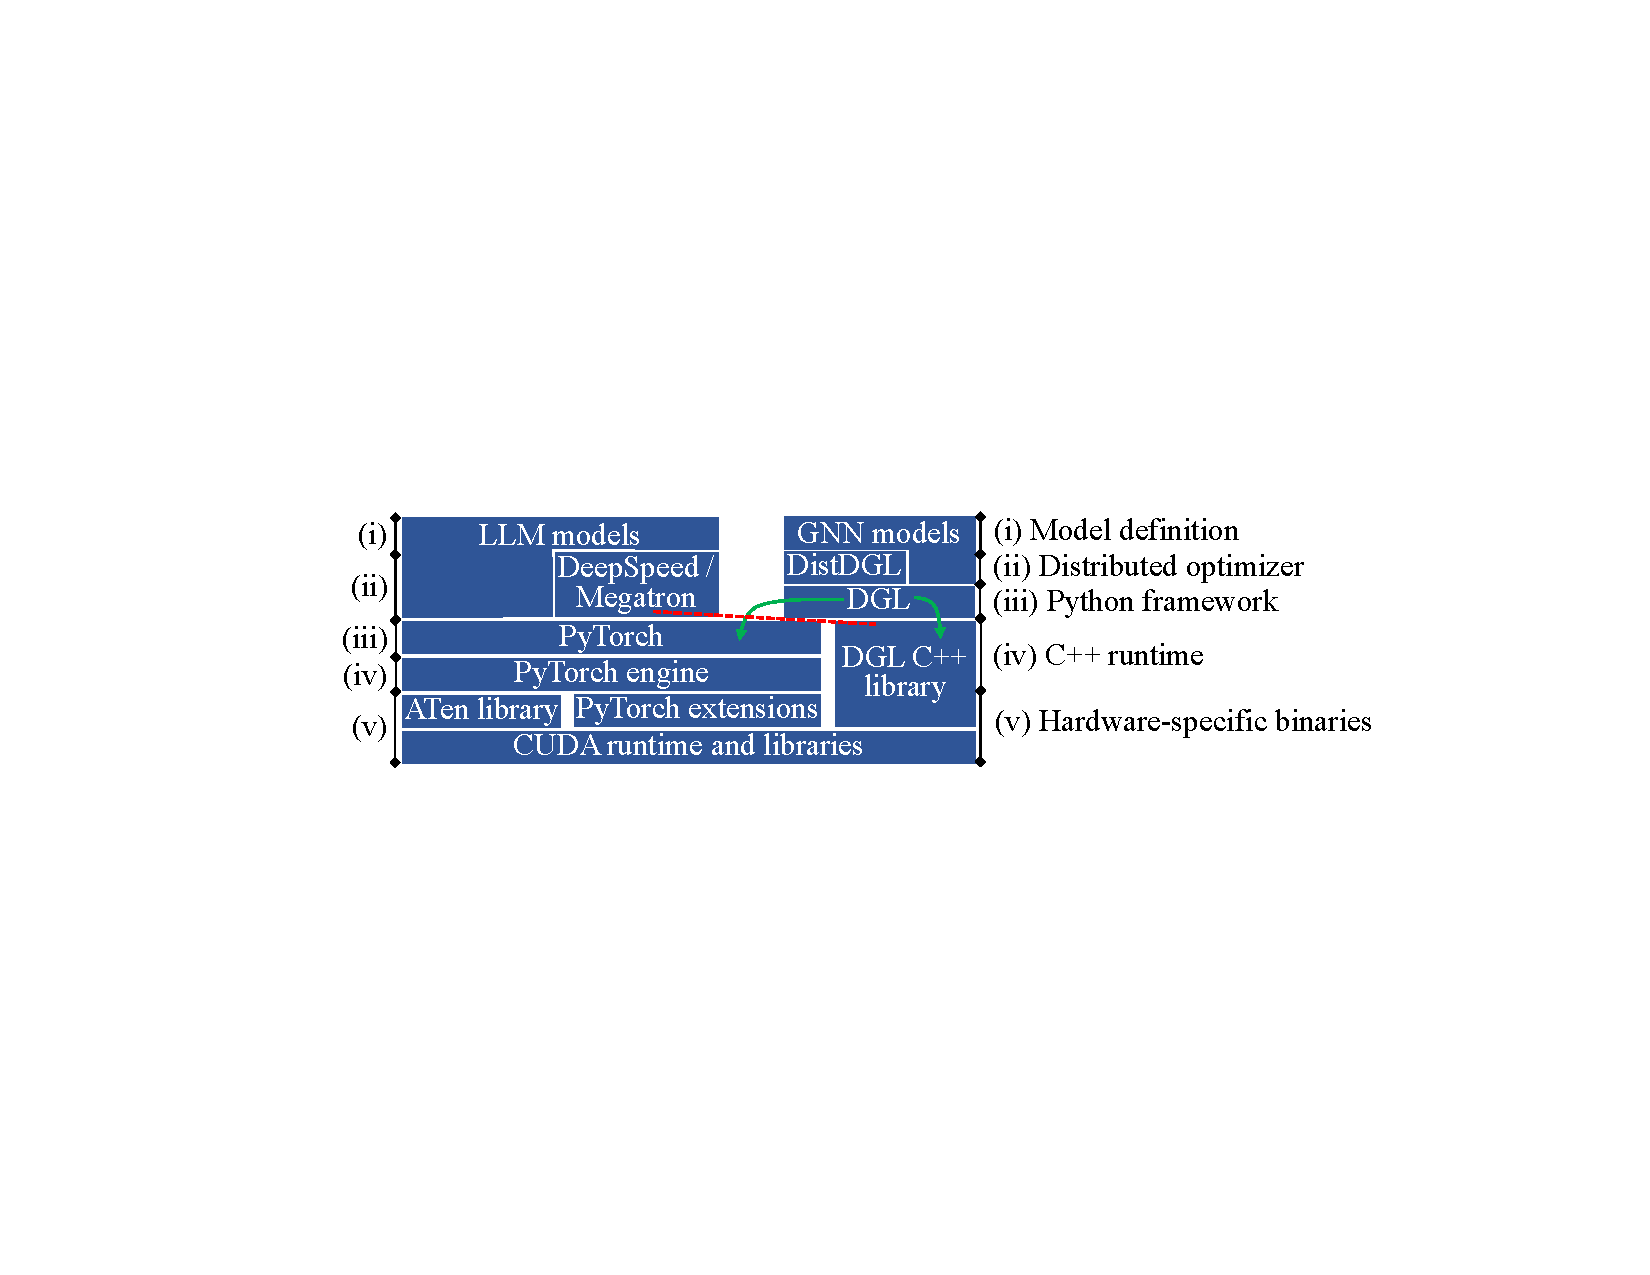
\includegraphics[width=0.85\linewidth]{figures/Intro/pytorch_stack.pdf}
    \caption{The PyTorch computing stack for GNN workloads and LLM workloads. As the GNN framework, Deep Graph Library~(DGL) calls PyTorch \kwc{functions} and functions provided by DGL C++ libraries~(green arrow). The LLM distributed optimizers, DeepSpeed and Megatron, do not rely on the DGL C++ library~(red dashed line). }
    \label{fig:pytorch_stack}
\end{figure}


Notice that users only need to define the forward propagation logic, as shown in Figure~\ref{lst:pytorch_nested_module}. PyTorch's auto-differentiation mechanism handles the computation of gradients without requiring users to manually specify the backward propagation logic. During forward propagation, PyTorch records \kwc{activations, i.e.,} the intermediate tensors, \kwc{and weights} required for backward propagation and constructs the corresponding computational graph. \kwc{In Figure~\ref{fig:pytorch_graph}, for example, \texttt{y} and \texttt{y\_expected} are the activations stored for  the backward propagation process of \texttt{MSELoss}, \texttt{MSELossBackward}}. During backward propagation, PyTorch executes the backward-propagation computational graph. PyTorch calls precompiled kernels to execute operators in forward propagation and backward propagation.


Another way to provide auto differentiation uses just-in-time~(JIT) compilation. For example, to perform auto differentiation, JAX 1)~captures the forward propagation functions' IR through trace-based JIT, 2)~generates the gradient functions' IR via transformation, and 3)~compiles CUDA binaries using XLA~\cite{joergAutomatedGPUKernel2019}. Similar\kwc{ly,} JIT-based approaches are adopted by PyTorch JIT~\cite{pengwuWorkshopsASPLOS_2024README}, Mathematica~\cite{dakkakCompilingHighlevelScripting2020}, Zygote~\cite{zygoteFluxMLZygoteJl2019}, CLAD~\cite{ioanaifrimGPUAccelerationAutomatic2021}, and Enzyme~\cite{mosesReversemodeAutomaticDifferentiation2021}.

Figure~\ref{fig:pytorch_stack} shows the PyTorch computing stack for GNNs and LLMs, the primary workloads addressed in this dissertation. At the top of the stack are the GNN models and LLM models. Users can use distributed optimizers, e.g., DeepSpeed for LLMs and DGL for GNNs. Both single-GPU execution and distributed optimizers are built on top of PyTorch, although DGL also relies on its library for graph-related operations. At the bottom of the stack are the CUDA runtime and math libraries. The stack \kwc{comprises} five layers from the top to the bottom: (i)~Model definition specifies the model architecture and pre-trained parameters. (ii)~Distributed optimizers provide mechanisms for device-level parallelism and communication. (iii)~Python frameworks offer layer definition, dataloading, and profiling utilities. (iv)~The C++ runtime provides a GIL-free context, auto differentiation mechanism, and functionality of operator dispatching. (v)~Hardware-specific binaries \kwc{provide the binaries to execute operators on devices. These binaries may} leverage vendor-optimized libraries and provide support for new hardware, e.g., tensor cores on Nvidia GPUs. \kwc{At this level, support for new operators can be added to the stack by creating new PyTorch extensions and registering them during runtime. PyTorch extensions use \texttt{pybind11}}~\cite{wenzeljakobPybindPybind112016} \kwc{to allow the new C++ code to interact with the Python runtime.}
